\documentclass{sigplanconf}

% The following \documentclass options may be useful:
%
% 10pt          To set in 10-point type instead of 9-point.
% 11pt          To set in 11-point type instead of 9-point.
% authoryear    To obtain author/year citation style instead of numeric.

\usepackage{amsmath}
\usepackage{listings}
\usepackage{subfigure}
\usepackage{graphics}
\usepackage{epsfig}
\usepackage{bbding}
\usepackage{color}
\usepackage{url}
\usepackage{xspace,amsthm,amsmath,amssymb,url,microtype,amsfonts,color}
\usepackage{graphicx,subfigure}
\usepackage{amscd,hyperref}
\usepackage{enumitem}
\usepackage{lstlang0}
\usepackage{fancyvrb}

\newcommand{\reals}{\mathbb{R}}
\newcommand{\prob}[1]{\Pr\left[#1 \right ]}
\newcommand{\expec}[1]{{\mathbb E}\left[#1 \right ]}
\newcommand{\var}[1]{{\mathbb V}\left[#1 \right ]}
\newcommand{\err}{{\mathcal E}}
\newcommand{\comment}[1]{\marginpar{!!!}{[\emph{#1}]}}

\newcommand{\checkcell}{\textsc{CheckCell}}

\DeclareMathOperator{\argmin}{argmin}
\DeclareMathOperator{\coeff}{coeff}
\DeclareMathOperator{\poi}{Poi}

\newtheorem{definition}{Definition}
\newtheorem{theorem}{Theorem}[section]
\newtheorem{proposition}{Proposition}[section]
\newtheorem{corollary}{Corollary}[section]
\newtheorem{lemma}{Lemma}[section]
\newtheorem{conjecture}{Conjecture}[section]
\newtheorem{fact}{Fact}
\newtheorem{problem}{Problem}
\newtheorem{example}{Example}
\newtheorem{claim}{Claim}

\begin{document}

\conferenceinfo{PLDI '13}{June 16--21, 2013, Seattle, Washington, USA}
\copyrightyear{2013} 
\copyrightdata{[to be supplied]} 

% \titlebanner{banner above paper title}        % These are ignored unless
% \preprintfooter{short description of paper}   % 'preprint' option specified.

\title{\checkcell{}: Data Debugging for Spreadsheets}

\authorinfo{\emph{authorship list omitted for anonymity}}

%\authorinfo{Daniel W. Barowy\and Dimitar Gochev\and Emery D. Berger}
%           {Department of Computer Science \\
%           University of Massachusetts, Amherst \\
%           Amherst, MA  01003}
%          {\{dbarowy,gochev,emery\}@cs.umass.edu}

\maketitle

\begin{abstract}
Testing and static analysis tools can help root out bugs in programs,
but not bugs in data. Checking data for errors is arguably as
important as finding program errors, but lacks effective tool
support. This paper introduces \emph{data debugging}, an approach that
combines dataflow dependence analysis with statistical analysis to
locate likely data errors. Since it is impossible to know \emph{a
priori} whether data are erroneous or not, data debugging does the
next best thing: locating data where an error would have the most
impact. Data debugging is particularly promising in the context of
data-intensive programming environments like databases and
spreadsheets, which intertwine data with programs (in the form of
queries or formulas).

This paper presents an implementation of data debugging in an add-in
tool for Microsoft Excel called \checkcell{}. \checkcell{} highlights
unusually impactful values in shades of red proportional to their
effect on the spreadsheet's computation (including charts and 
formulas). \checkcell{} is efficient: its algorithms are asymptotically
optimal, and it takes under a minute to run on large spreadsheets. A
user study verifies the effectiveness of data debugging to find
data errors. \checkcell{} users were able to find errors with XX\%
accuracy, while users without were only able to achieve YY\% accuracy.

\end{abstract}

%\category{CR-number}{subcategory}{third-level}

%\terms

%\keywords

\section{Introduction}
% \textbf{Software bugs: well-studied, effective tools.}
In many computational tasks, correctness is a primary concern. Most
work in the programming language community over the past decades has
focused on ways to discover whether the program performing the computation is
correct. Techniques to reduce program errors range from
testing~\cite{unittesting,fuzztesting} and runtime
assertions~\cite{samanderansthing,others}, to dynamic and static
analysis tools that can discover a wide range of
bugs~\cite{valgrind,dawsonthing,otherpcmemberfoo}. Using these
approaches and tools greatly increases the ability of programmers to
find errors and reduce their impact, contributing to improving overall
code quality.

% Data errors, not so much.
However, a program is just one part of a computation. When its input
has errors, the result of the computation is likely to not be
correct. Data errors can arise in a number of ways, including mistakes
in data entry or corrupted data sources. Unlike programs, data cannot
easily be checked for correctness.

% \textbf{Data errors really important in data-intensive programming environments.}

While data errors pose a threat to the correctness of any computation,
they are especially problematic in data-intensive programming
environments like databases, spreadsheets, and certain scientific
computations (e.g., data analysis using R~\cite{FIXME}). In these settings,
data correctness can be as important as program correctness (``garbage
in, garbage out''). The results produced by the
computations---queries, formulas, charts, and other analyses---can end
up being rendered invalid by data errors. These errors can be costly:
for example, spreadsheet errors have led to losses of millions of
dollars~\cite{FIXME}.

%%%%  Things to add in citations: %%%%
% TransAlta took a $24 million charge -- copy and paste error
% http://www.skillsportal.co.za/page/training/articles/512049-Spreadsheet-errors-can-be-a-major-cost-to-your-business#.UJbfX2l250s
% http://www.flintshirechronicle.co.uk/flintshire-news/local-flintshire-news/2010/02/18/flintshire-county-council-school-cash-blunder-down-to-spreadsheet-error-51352-25856321/
% http://binnenland.nieuws.nl/566978


% cite approximate computation stuff?

By contrast with the proliferation of tools at a programmer's disposal
to find program errors, few tools exist to help find data errors. Part
of the problem is that, unlike program errors, it is more difficult to
decide whether any given data element is an error or not. For example,
the number \texttt{132} might be correct, or it could be a
transposition error from \texttt{123}. More insidiously, a misplaced
or omitted decimal point could change a data item by orders of
magnitude. Unfortunately, manual data auditing to find this kind of
mistake is both onerous and difficult to scale up to even the moderate
size of data in spreadsheets.


% \textbf{Existing approaches don't really work.}

Existing approaches to finding data errors include
statistical \emph{outlier detection} and \emph{data cleaning}. Outlier
detection can be used to find errors only when the input data follows
a known distribution (e.g., Gaussian). Automatic identification of
data distributions is error-prone and can give rise to an excessive
number of false positives. Data cleaning primarily copes with errors
in databases via cross-validation with ground truth data, which may
not exist.

\subsection*{Contributions}

This paper presents an approach to locating likely data errors that we
call \emph{data debugging}. Data debugging leverages the fact that in
data-intensive programming environment like spreadsheets or databases,
data and programs (e.g., queries or formulas) are intertwined.

%, data debugging reframes the problem to find data
%whose presence has an unusually large impact on the computation as a
%whole.

Data debugging uses static and dynamic analysis to guide a statistical
process that isolate data whose impact dramatically affects the final
results of a computation. It first builds a dependency graph of
the program, and then systematically measures the effect of re-running
the computation after replacing data items with other items drawn
randomly from the same input set.

By calling attention to data that has an unusually large impact on the
final computation, data debugging provides insights into both the data
and the computation and can reveal errors. Since it is impossible to
know \emph{a priori} whether data are erroneous or not, data debugging
does the next best thing: locating data where an error would have the
most impact. Intuitively, data that has an unusually high impact on
the final result is either very important or it is wrong. By
contrast, data that is wrong but whose presence or absence has little
impact on the final result does not merit special attention.

This paper presents the first tool for data debugging that operates in
the context of spreadsheets. This system, called \checkcell{}, works
as a plug-in for Microsoft Excel, though its principles are broadly
applicable. \checkcell{} builds a dependency graph of the entire
computation represented by a spreadsheet, where outputs and
intermediate nodes include formulas and charts, and where data cells
form the leaves. \checkcell{} then performs a statistical perturbation
analysis of the effect of inclusion or exclusion of individual cells,
measuring their impact on the spreadsheet's outputs by recalculation
on the perturbed inputs. \checkcell{} then ranks by influence all
data whose effect crosses a threshold of unusualness. In the user
interface, \checkcell{} colors the cells containing this data in
shades proportionally to their impact: the more impact, the brighter
the highlighting.

\checkcell{} is efficient: it operates in time linear in the number
of data elements, which is optimal. The current prototype is untuned
but analysis time is generally low, taking less than a minute to run
on spreadsheets containing thousands of cells. A user study verifies
the hypothesis that data debugging's approach of identifying data with
unusual impacts is effective at locating errors. With \checkcell{}'s
help, users were able to find XX\% of injected errors, while users
without \checkcell{} were only able to find YY\% of errors.

%We have developed a Microsoft Excel extension, or add-in, written in
%C\#, which uses cross-validation techniques and perturbation analysis
%to look for numerical values that appear suspicious.  Values that
%appear to be potential errors are highlighted proportionally to the
%likeliness that they are incorrect, as judged by our analysis -- the
%more likely a value is to be wrong, the brighter the highlighting.


\section{Background}
\label{sec:background}
Background.


\section{Overview}
\label{sec:overview}
This section provides an overview of how data debugging
works. Section~\ref{sec:algorithm} describes the algorithms in full
detail, and Section~\ref{sec:analysis} includes formal analysis of various
aspects of data debugging, including asymptotic performance and
statistical effectiveness.

\paragraph{Dependence Analysis.}
The first step in data debugging is to identify the relationship of
data (inputs) to computations (outputs). For example, in a database
management system, data inputs would be tuples (records) and computations would
be queries. In a spreadsheet, inputs are data in cells, while
computations are either terminal formulas (not used by other formulas)
or charts.

\paragraph{Impact Analysis.}
The next step is to iterate through the data itself to test the impact
of each data item on all computations. For each item, data debugging
repeatedly chooses a random other item from the same ``distribution'',
e.g., another tuple in the same table, or another cell in the same
range, and replaces the item being tested with the randomly-selected
one.

The computations are then recalculated using this new dataset. Changes
in the computations are recorded as their \emph{impact scores} on each
data item.  The impact score for a computation depends on whether the
output is numeric or non-numeric. For numeric data, the impact score
is the normalized change to the original value.
For non-numeric data, the impact score is an \emph{indicator value}: 1
if the result of the computation changed, and 0 if not.

% Each data item maintains a separate impact score for every computation.

This process is repeated some fixed number of times, accumulating the
impact scores associated with each datum. To ensure a high level of
statistical confidence, this number should be around 30. The impact
score is then divided by the number of iterations, resulting in an
average absolute deviation for each data item's impact.

\paragraph{Impact Scoring.}
Finally, the impacts of each data item are normalized by transforming
them into absolute z-scores, where $|z|$ is the absolute distance of
each item from the sample mean, divided by the sample standard
deviation. Each data item's absolute z-scores are then averaged across
all the outputs, and data debugging assigns that average as the
\emph{overall impact score} of each data item. The overall impact
score represents the average distance from the mean impact, in numbers
of standard deviations. Note that this interpretation does not depend
on normality assumptions about the data or its impact; in fact, using
the normal distribution to rank impacts is conservative, as
Section~\ref{sec:analysis} explains.

Intuitively, data with large overall impact scores either have an
extremely high impact on a small number of computations, or a high
impact on a large number of computations. The overall impact score can
be used both for ranking and for displaying the relative anomalousness
of the impact of particular data items, e.g., by coloring such values
in brighter colors corresponding to their distance from the mean. It
also makes it straightforward to decide how many data to report. A
standard approach, which we adopt here, is to stop reporting data once
it falls below two standard deviations away from the mean,
corresponding to more than a 95\% level of confidence that these are
outliers.


% ``score'' the impact by highlighting the values proportional to their z-score

% we just need to report outliers in the impact. assuming the impacts
% are normal is a conservative approach: the normal has 0 skewness
% (skew = distribution around the mean -- normal is symmetric, so 0
% skew) and low (either 0 or 3) kurtosis, depending on your definition
% of kurtosis. Every non-normal distribution is by definition more skewed and most
% distributions have a higher kurtosis (heavier tails), so we may
% overmark outliers. We won't find outliers in distributions with
% negative kurtosis, but those are super weird (no tails -- they drop
% below the x-axis at some point on either side), so it's hard to
% argue that they have outliers at all.



\section{Algorithm}
\label{sec:algorithm}
\subsection{Motivating Example}

Small input errors can have dramatic consequences in the correctness of certain computations.  Misplaced decimal points and erroneously omitted or inserted digits can affect the accuracy of a calculation by an order of magnitude.  A mistyped digit can also have large effects if a calculation is sensitive to small changes.  All of these errors are the result of a single typographical error.  One study found that the average error typographical error rate to be as high as 24\% for user logins~\cite{Robinson:1998:CUV:2229220.2229465}.  Sufficiently large spreadsheets are nearly guaranteed to contain at least one error.

Figure~\ref{fig:personal_budget} is a typical spreadsheet to track one's personal expenses over the course of a month.  A simple calculation performed at the end of the month informs the user whether they can afford a luxury item, such as an expensive dinner.  The calculation answers ``yes'' if the user's monthly expenses were at least \$150 under budget.  However, this example contains a simple typographical error which results in the wrong answer.

\begin{table}[t!]
  \centering
    \begin{tabular}{|c|r|r|r|}
    \hline
    & \myalign{c|}{\textsf{\bf{A}}} & \myalign{c|}{\textsf{\bf{B}}} & \myalign{c|}{\textsf{\bf{C}}} \\
    \hline
    \textsf{\textsf{\bf{1}}} & \textsf{MONTHLY BUDGET} & \textsf{Projected Cost} & \textsf{Actual Cost} \\
    \hline
    \textsf{\textsf{\bf{2}}} & \textsf{Rent} & \textsf{\$1150}  & \textsf{\$1150} \\
    \hline
    \textsf{\textsf{\bf{3}}} & \textsf{Phone} & \textsf{\$3675}  & \textsf{\$36.75} \\
    \hline
    \textsf{\textsf{\bf{4}}} & \textsf{Gas} \& \textsf{Electricity} & \textsf{\$80}    & \textsf{\$87.23} \\
    \hline
    \textsf{\textsf{\bf{5}}} & \textsf{Waste removal} & \textsf{\$11.25} & \textsf{\$11.25} \\
    \hline
    \textsf{\textsf{\bf{6}}} & \textsf{Groceries} & \textsf{\$200}   & \textsf{\$187.81} \\
    \hline
    \textsf{\textsf{\bf{7}}} & \textsf{Car payment} & \textsf{\$225}   & \textsf{\$225} \\
    \hline
    \textsf{\textsf{\bf{8}}} & \textsf{Gasoline} & \textsf{\$50}    & \textsf{\$62.3} \\
    \hline
    \textsf{\textsf{\bf{9}}} & \textsf{Clothing} & \textsf{\$100}   & \textsf{\$59.99} \\
    % \hline
    % \textsf{\textsf{\bf{10}}} & \textsf{Total} & \textsf{\$5491.25} & \textsf{\$1820.33} \\
    \hline
    \textsf{\textsf{\bf{10}}} & \textsf{Fancy dinner tonight?} & \textsf{Yes}   &  \\
    \hline
    \end{tabular}%
  \caption{A sample spreadsheet showing a personal budget, with a decimal point typo in cell \texttt{B3}.\label{fig:personal_budget}}
\end{table}%
  
The erroneous value in cell B3 changes the answer to the question ``Can I afford a fancy dinner?''.  Even for users whose typographical error rate is low, the likelihood of making at least one such error increases as the spreadsheet grows in size.  Can automated analysis be of any assistance?

\subsection{Dependency Analysis}

The formula in cell B10 computes whether an expensive dinner is a good idea given the difference between projected cost and actual cost: \texttt{=IF(SUM(B2:B9)-SUM(C2:C9) > 150, ``Yes'', ``No'')}.  Without knowing something about this domain \emph{a priori}, it is difficult to conclude that it might be an error.

Fortunately, the structure of spreadsheet calculations provides valuable information.  While the spreadsheet model of computation appears to be quite different from traditional computer programs, these differences are largely superficial.  Both forms of computation possess functions with input, output, and conventional control flow structures.  As such, we can represent the dataflow graph of a spreadsheet in a manner similar to traditional programs.  Spreadsheet formulae in Microsoft Excel are pure, and there is no facility for looping constructs, thus the dataflow graph under consideration is a directed acyclic graph (DAG).

% DWB: mention control-flow constructs? %
A spreadsheet's dataflow graph helps \checkcell find a function's input distribution.  The dataflow graph for this calculation can be seen in Figure~\ref{fig:ex_compgraph}.  In the dataflow graph, inputs and outputs are represented as leaves in a DAG.  Intermediate nodes are functions.  Nearly all functions in Microsoft Excel take vectors as arguments.  \checkcell operates under the assumption that values in a vector are homogenous.  \checkcell additionally assumes that inputs are order-independent, however it does not need to assume that inputs are independent of each other.  Thus \checkcell is able to treat similar input values as samples of the same random variable.

By definition, an ``error'' is a value which does not belong to a random variable's distribution.  Thus outlier detection techniques appear to be a useful statistical tool for determining errors in an input.  However, two new difficulties immediately arise: 1) values in spreadsheets are not necessarily numerical, and 2) outlier detection techniques make strong assumptions about the distribution of the inputs.  \checkcell makes no assumptions about the datatype of the inputs.  E.g., string inputs are amenable to analysis.  Furthermore, \checkcell's analysis is nonparametric, and thus values from any distribution are acceptable.

\subsection{Impact Computation}

\checkcell reframes the problem of finding a statistical outlier to the problem of finding a value which has an unusual effect on a computation.  If an error occurs in a set of values, and the replacement of that value with the true value causes a dramatic change in the output of a function, the value is likely to be a bug.  In the absence of the true replacement value, which is unknown, \checkcell uses other values from the same distribution a a proxy.  Since the erroneous value, by definition, does not belong to the input distribution, its exclusion should have a statistically significant effect on the output distribution of the function.

Every value in a function's input distribution are perturbed by swapping it with representatives from the same distribution.  Since \checkcell cannot know \emph{a priori} which values of the input distribution should be used as proxies, all possibilities need to be considered.  To reduce computational overhead, the system described in this paper uses a sampling technique to choose candidate values for swapping.  For small inputs (i.e., input distributions with fewer than 30 values), the procedure degenerates to an exact statistical procedure.  This technique is analyzed in detail in section~\ref{FIXME}.

The output of systematic value perturbation is a vector of impact distributions, one distribution for each value.  \checkcell computes the average value of each of these impact distributions and poses the following question: which impact is an outlier?  By the central limit theorem (CLT), the distribution of average values converges to the normal distribution ~\cite{FIXME}.

The CLT's convergence guarantee requires that the random variable under consideration be identically distributed.  Thus outlier rejection techniques, which are designed to find values which do not belong to a distribution, can be used to find the values which cause the average-impact distribution to deviate from normality.  \checkcell uses Peirce's criterion for outlier rejection to flag these values.  In contrast with other outlier rejection procedures, Peirce's criterion will execute until it has removed a sufficient number of values to restore normality to a distribution.  This means that \checkcell will find all values that have an unusual influence.

It is informative to compare \checkcell's treatment of ``data bugs'' with the approaches for finding bugs in code.  Data races are notoriously difficult to find in multithreaded code, and many tools have been developed to find them~\cite{FIXME}.  However, tools which focus their efforts on finding all possible data races overwhelm programmers with their verbosity.  The important races to find are the ones that materially affect the output of a computation.  All other races are benign.  \checkcell operates under a similar principle, which is that data errors which affect the output of a computation are the ones that should be considered.

\section{Evaluation}
\label{sec:evaluation}

\begin{table*}[!t]
  \centering \begin{tabular}{l|rrr||r|rrr}
 \small{\bf{Spreadsheet}} & \small{\bf{Formulas}} & \small{\bf{Cells}} & \small{\bf{Cells}} & \small{\bf{Runtime}} & \small{\bf{Dep.}} & \small{\bf{Impact}}   & \small{\bf{Impact}} \\
 & & {\small{\it{raw}}} & {\small{\it{weighted}}} & \small{\it{total (s)}} & \small{\bf{Analysis}} & \small{\bf{Analysis}} & \small{\bf{Scoring}} \\
\hline
\small{3660 schedule S2003} & \small{31} & \small{1} & \small{0} & \small{1.54} & \small{0.73} & \small{0.44} & \small{0.34} \\ 
\small{ReqComp} & \small{54} & \small{162} & \small{0} & \small{1.95} & \small{0.95} & \small{0.52} & \small{0.44} \\ 
\small{Inventory\_Control} & \small{33} & \small{21} & \small{0} & \small{4.71} & \small{1.67} & \small{1.59} & \small{1.42} \\ 
\small{RMRanker95} & \small{79} & \small{54} & \small{11} & \small{7.07} & \small{2.74} & \small{2.38} & \small{1.91} \\ 
\small{Logistikkostnader} & \small{73} & \small{29} & \small{26} & \small{8.88} & \small{3.48} & \small{2.97} & \small{2.40} \\  
\small{HMWK112403} & \small{36} & \small{41} & \small{27} & \small{2.31} & \small{0.88} & \small{0.78} & \small{0.63} \\ 
\small{30day} & \small{125} & \small{92} & \small{30} & \small{3.01} & \small{1.39} & \small{1.31} & \small{0.27} \\ 
\small{2002fairreport} & \small{3} & \small{39} & \small{39} & \small{4.30} & \small{1.29} & \small{1.67} & \small{1.30} \\ 
\small{9620040303160820} & \small{42} & \small{81} & \small{81} & \small{4.77} & \small{1.19} & \small{2.74} & \small{0.81} \\  
\small{Inventory errors} & \small{100} & \small{129} & \small{90} & \small{2.83} & \small{1.25} & \small{1.02} & \small{0.53} \\ 
\small{grades} & \small{227} & \small{661} & \small{96} & \small{154.45} & \small{3.06} & \small{149.85} & \small{1.51} \\ 
\small{expenses\_ans} & \small{57} & \small{60} & \small{120} & \small{3.24} & \small{0.92} & \small{2.15} & \small{0.15} \\ 
\small{grades2002} & \small{61} & \small{143} & \small{123} & \small{2.67} & \small{1.03} & \small{1.11} & \small{0.51} \\ 
\small{csDept-PayrollTimecardEntry} & \small{68} & \small{204} & \small{124} & \small{7.37} & \small{1.85} & \small{4.37} & \small{1.10} \\  
\small{Example\_3} & \small{71} & \small{130} & \small{127} & \small{3.15} & \small{1.22} & \small{1.56} & \small{0.28} \\ 
\small{lmc\_financial} & \small{72} & \small{148} & \small{142} & \small{17.15} & \small{4.69} & \small{7.63} & \small{4.80} \\ 
\small{104r} & \small{22} & \small{146} & \small{144} & \small{6.66} & \small{1.81} & \small{3.26} & \small{1.54} \\ 
\small{TRAIL INVENTORY N\#A850A} & \small{2} & \small{156} & \small{156} & \small{6.15} & \small{1.12} & \small{3.99} & \small{0.99} \\ 
\small{Grades-6\_excerpt} & \small{106} & \small{168} & \small{168} & \small{1.83} & \small{1.10} & \small{0.45} & \small{0.25} \\ 
\small{intresults} & \small{1066} & \small{3158} & \small{239} & \small{318.91} & \small{17.12} & \small{287.63} & \small{14.12} \\ 
\small{OakProducts} & \small{69} & \small{271} & \small{242} & \small{6.82} & \small{1.67} & \small{4.20} & \small{0.91} \\ 
\small{am\_skandia\_fin\_supple\#A80EE} & \small{56} & \small{272} & \small{268} & \small{6.64} & \small{1.53} & \small{4.01} & \small{1.06} \\ 
\small{E04\_AppE\_Census\_Database\_50} & \small{42} & \small{300} & \small{300} & \small{39.04} & \small{4.07} & \small{32.72} & \small{2.22} \\ 
\small{pfi-anxa} & \small{5} & \small{310} & \small{310} & \small{73.56} & \small{16.38} & \small{33.10} & \small{24.05} \\ 
\small{q exhibit54-OEA} & \small{797} & \small{1160} & \small{365} & \small{102.56} & \small{18.03} & \small{68.70} & \small{15.79} \\ 
\small{econ424-fall2003-publ\#A8A23} & \small{93} & \small{517} & \small{384} & \small{62.83} & \small{3.91} & \small{56.96} & \small{1.93} \\ 
\small{Grades\_EEE481\&581} & \small{177} & \small{757} & \small{756} & \small{40.11} & \small{3.31} & \small{35.74} & \small{1.03} \\ 
\small{gpa\_calculator} & \small{80} & \small{80} & \small{819} & \small{115.86} & \small{1.88} & \small{113.67} & \small{0.28} \\ 
\small{s446gradessp04} & \small{335} & \small{1369} & \small{1247} & \small{129.36} & \small{9.76} & \small{113.29} & \small{6.27} \\ 
\small{NEW} & \small{2626} & \small{2574} & \small{2403} & \small{683.32} & \small{115.75} & \small{440.30} & \small{127.23} \\ 
    \end{tabular}%
  \caption{The benchmark suite of 30 spreadsheets, a random sample from the EUSES repository~\cite{Fisher:2005:ESC:1082983.1083242}, ordered by weighted number of cells. The raw number of cells indicates the number of cells that are used in any formula; the weighted number of cells weighs each cell by the number of formulas that depend on it. A breakdown of \checkcell{} execution times (in seconds) appears on the right side.\label{tab:spreadsheet_characteristics}}
\end{table*}

We evaluate \checkcell{} across two dimensions: its execution time,
and its effectiveness at finding actual errors.

Our experimental platform is a 13'' MacBook Air equipped 4GB of RAM
and an Intel Core i5-2557M processor running at 1.70GHz. The operating
system is Windows 7 Professional (SP1), which executes non-virtualized
(via Bootcamp). \checkcell{} was compiled using Microsoft Visual C\#
2010, and runs as an add-in in Microsoft Excel 2010.

\subsection{Execution Time}
\label{sec:execution_time}

To measure the runtime of \checkcell{}, we run it on a random subset
of 30 spreadsheets drawn from the EUSES
corpus~\cite{Fisher:2005:ESC:1082983.1083242}, excluding those that do not contain
formulas.

Table~\ref{tab:spreadsheet_characteristics} includes characteristics
of these spreadsheets, ordered by the number of formulas each
contains. We include two columns that count the number of cells in
different ways. \emph{Cells (raw)} indicates the total number of cells
that participate in any computation. \emph{Cells (weighted)} indicates
the total number of cells, weighted by the number of times each cell
is used in a computation. For example, a cell that is involved in two
computations is counted twice.

\begin{figure*}[!t]
\centering
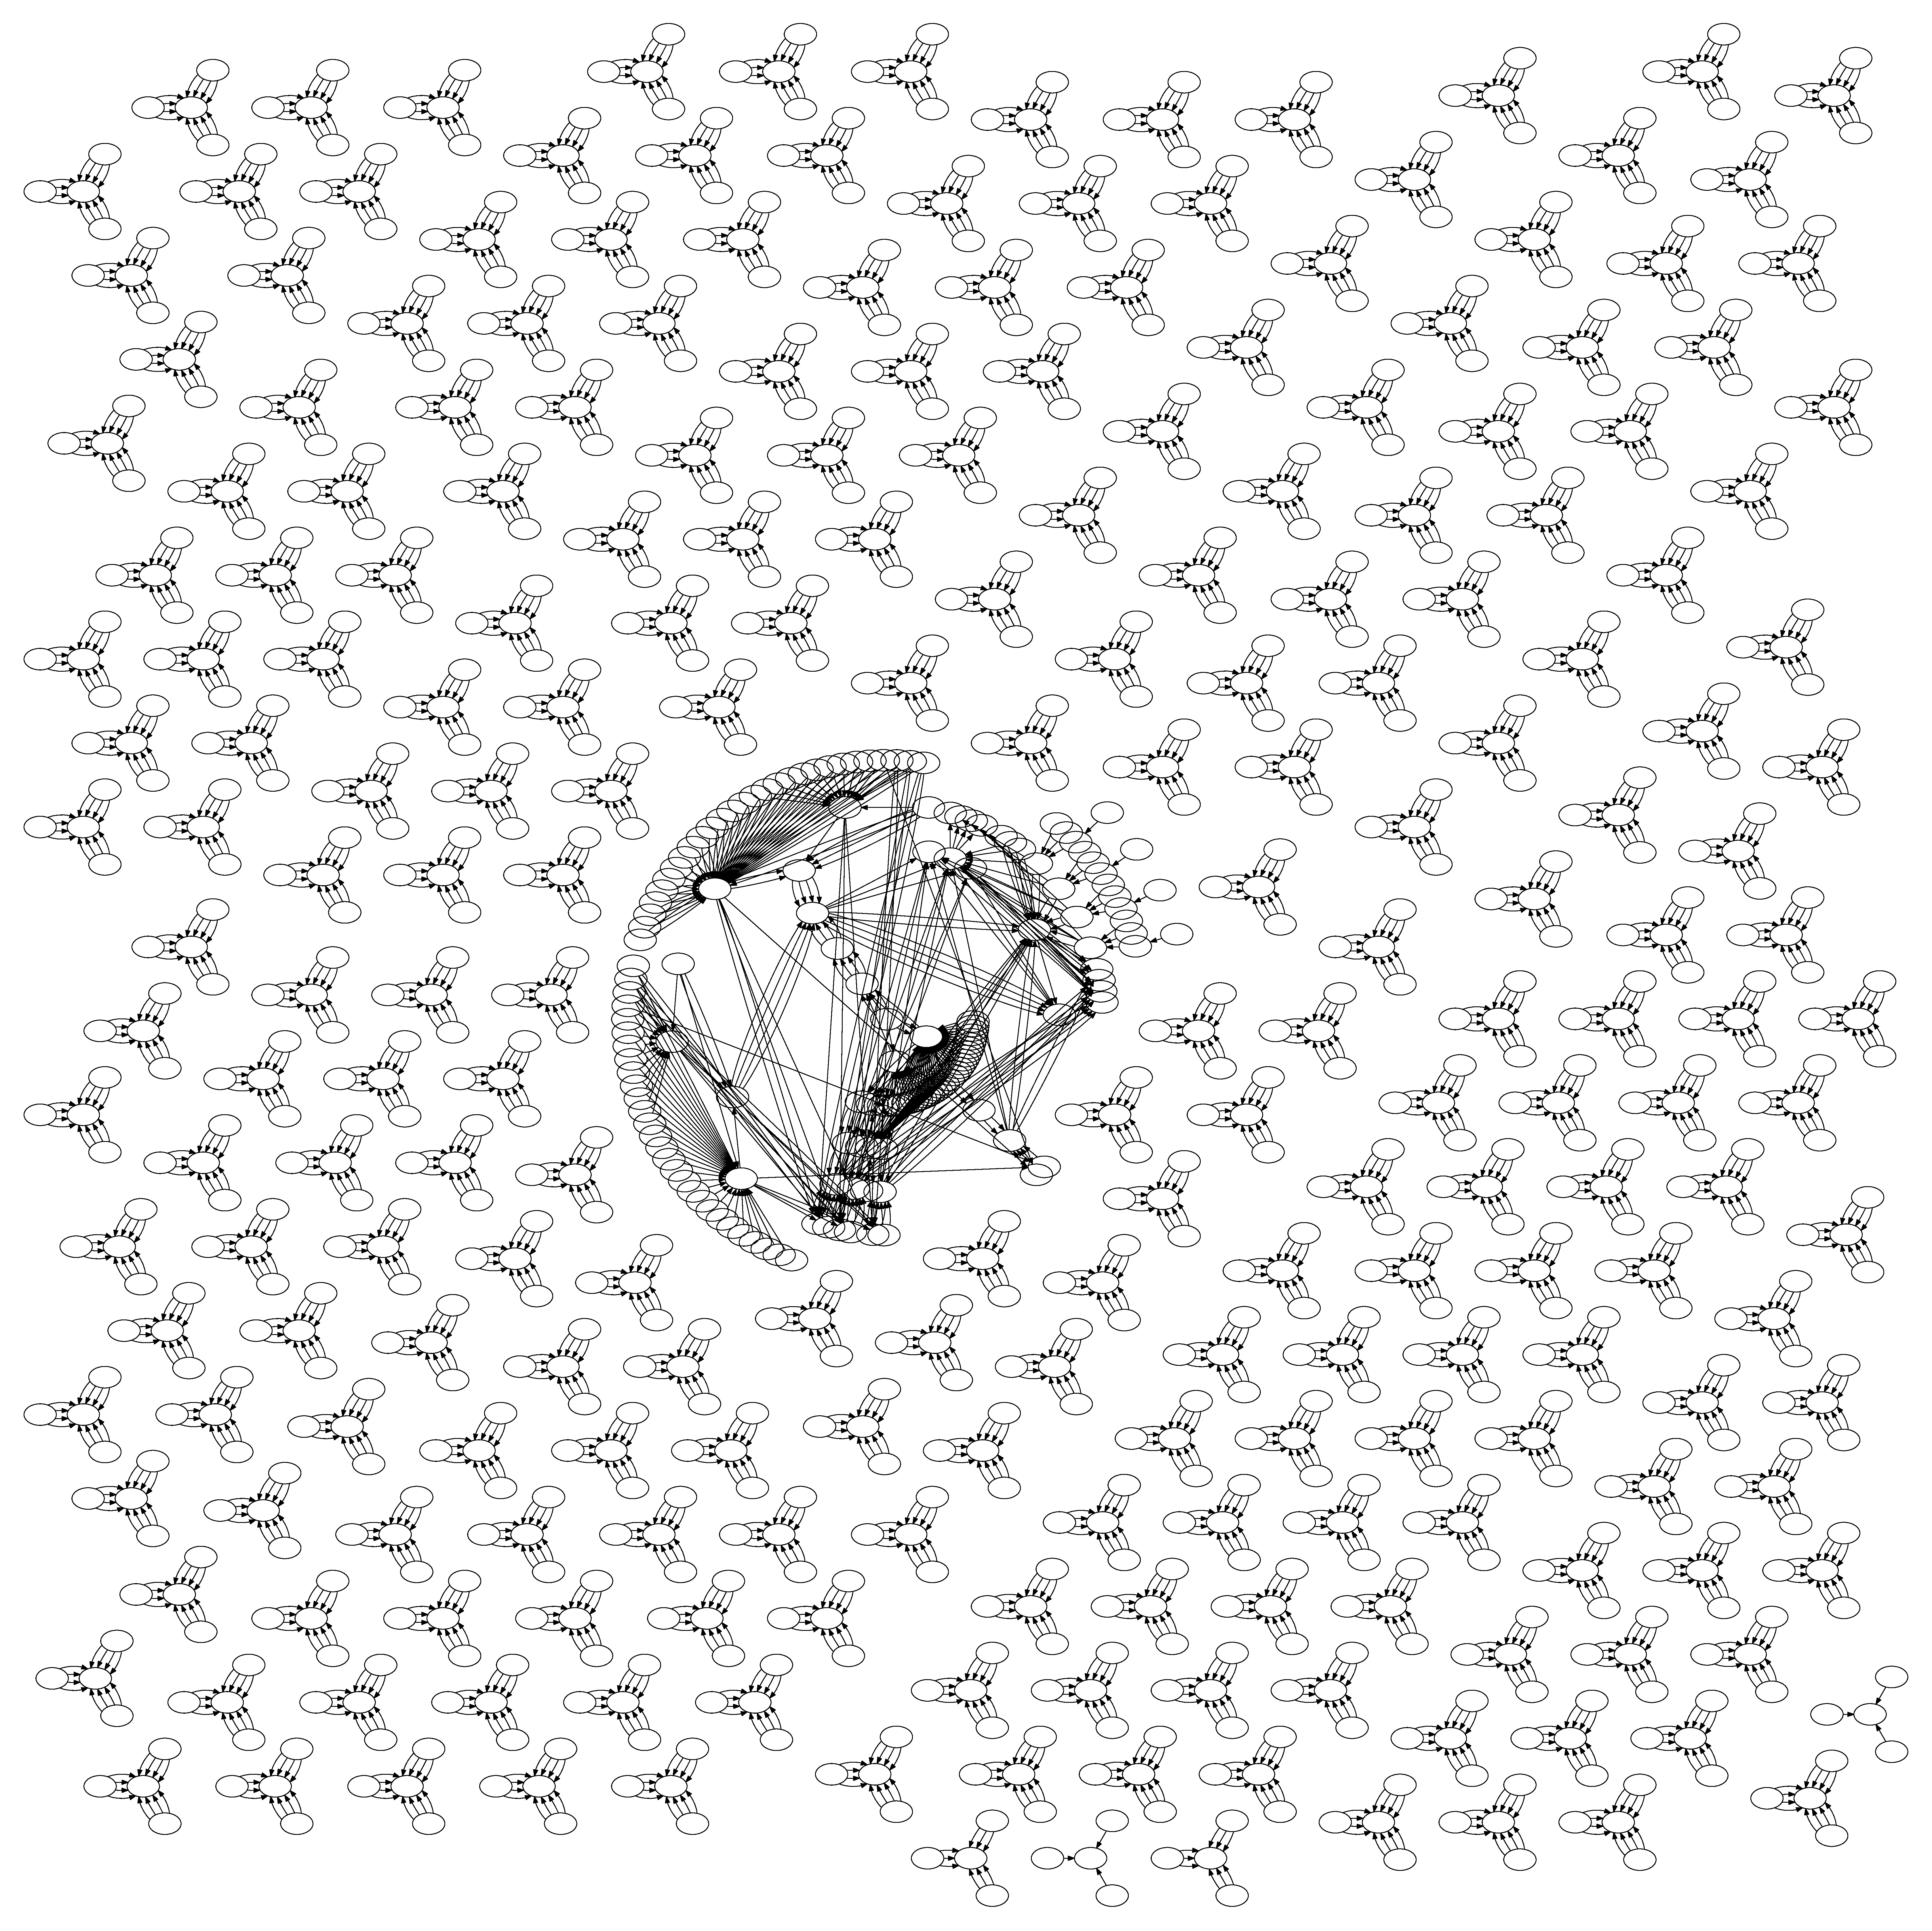
\includegraphics[width=7in]{intresults_tree}
  \caption{A dataflow graph for the \texttt{intresults} spreadsheet.  The highly-connected clique in the center causes the impact analysis to dominate \checkcell{}'s runtime. \label{fig:intresults_tree}}
\end{figure*}

\begin{figure*}[!t]
\centering
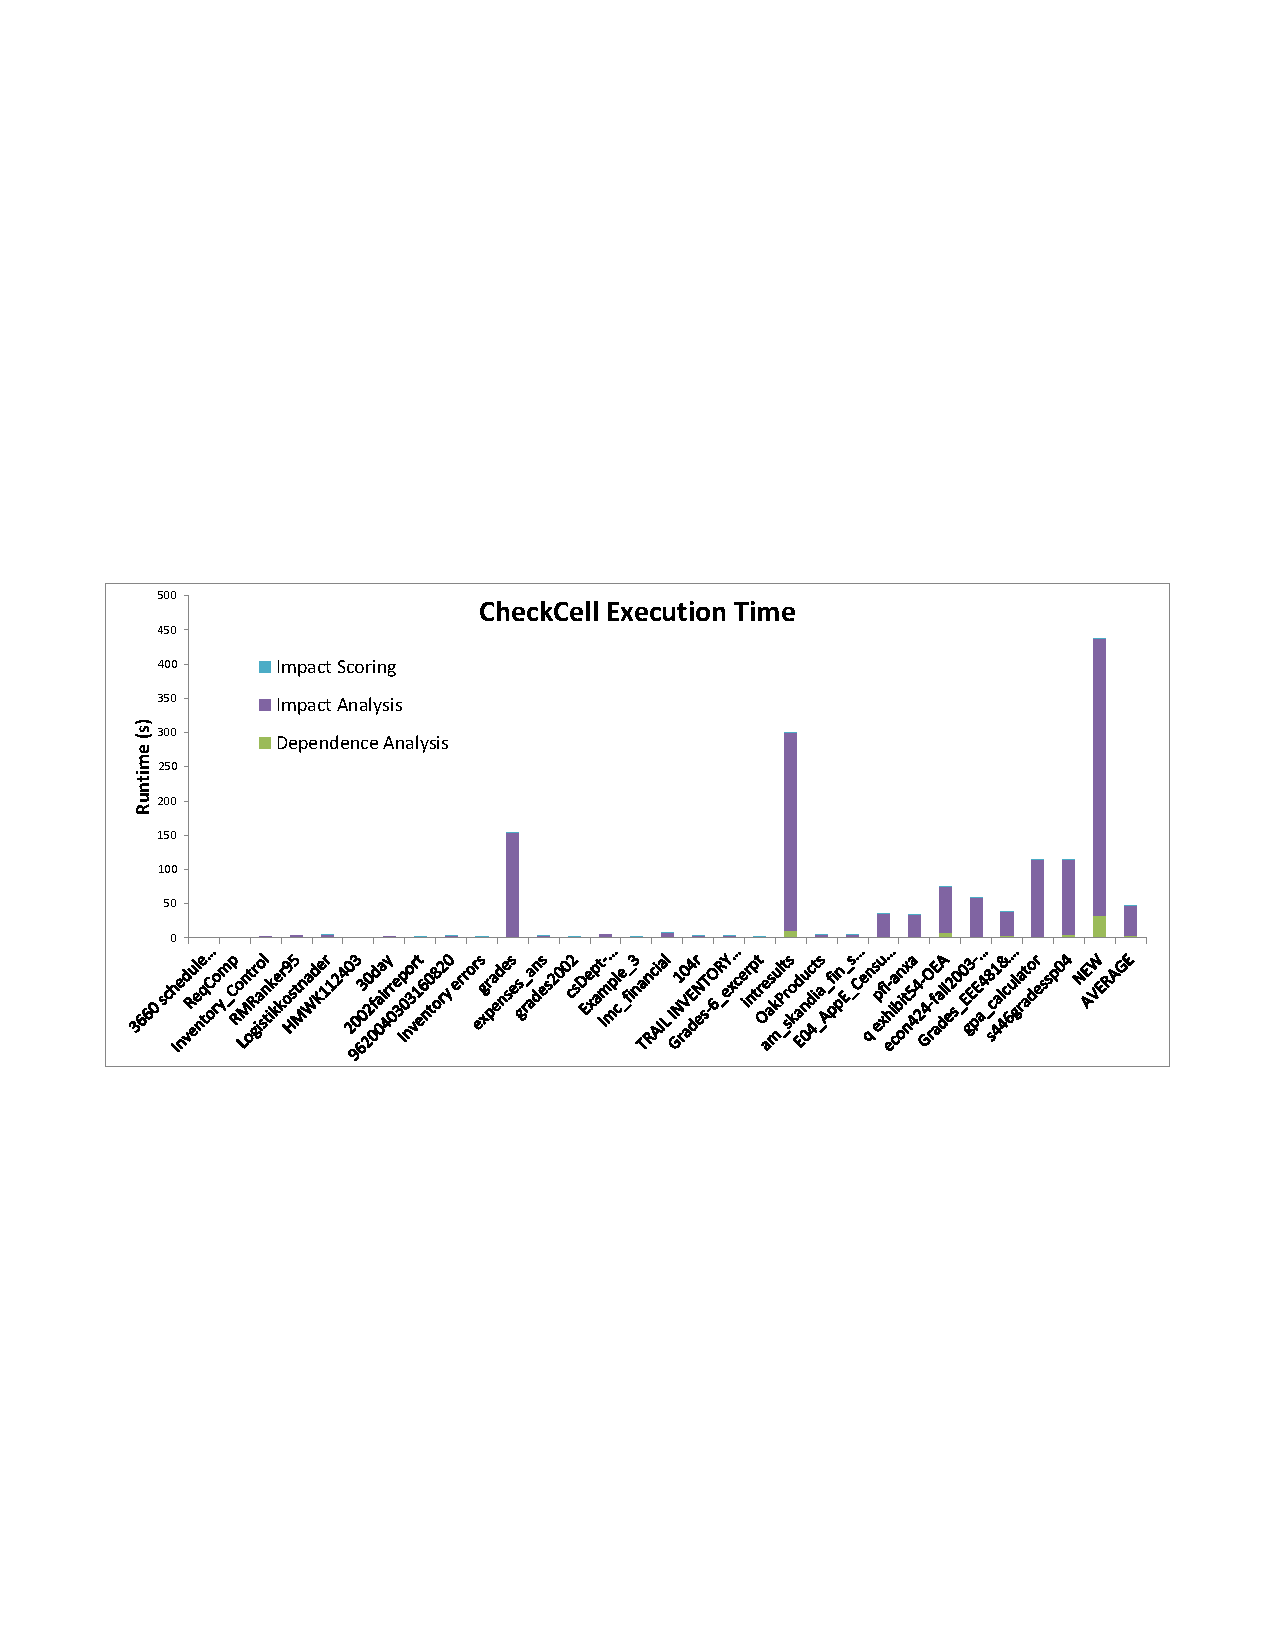
\includegraphics[width=5.5in]{execution_time_graph}
  \caption{\checkcell{} execution time. For most of the spreadsheets, \checkcell{} completes its analysis in under 9 seconds; for all but two, it completes in under three minutes (see Section~\ref{sec:execution_time}).\label{fig:execution_time_graph}}
\end{figure*}
 
Figure~\ref{fig:execution_time_graph} reports the performance of data
debugging across our spreadsheet suite, ordered by the weighted number
of cells. Table~\ref{tab:spreadsheet_characteristics} includes the full data.

For 19 of the 30 spreadsheets, \checkcell{} takes 9 seconds or less to
complete. Its runtime is less than three minutes for all but two of
the spreadsheets: \texttt{intresults} and \texttt{NEW}, which take 318
seconds and 683 seconds, respectively. The average runtime over all
spreadsheets is 61 seconds; without the two outliers, it is 29
seconds. As our analysis in Section~\ref{sec:asymptotic_analysis}
predicts, the cost of \checkcell{} is generally proportional to the
cost of the impact analysis, which is in turn dependent on the
weighted number of cells.

The spreadsheets that require the most execution time both have by far
the largest number of formulas (1,066 and 2,626), and the latter also
has the largest number of weighted cells (2,403). Their relatively
high execution time is attributable to the fact that cost of impact
analysis increases as the number of formulas increases, since the
Excel recalculation engine must do more work per item tested.

\paragraph{Summary:} For nearly every spreadsheet
 examined, \checkcell{}'s runtime is under three minutes; we believe
 this overhead is acceptable for an error detection tool.

% Info about the benchmarks.

% \subsection{Benchmarks}

%\subsection{Case Studies}

% \paragraph{9-Grades}

\subsection{Error Detection}
\label{sec:user_study}

While \checkcell{} can be used across the EUSES suite, looking for
errors in existing spreadsheets is problematic because we do not know
what the ground truth is. To evaluate \checkcell{}'s efficacy at
finding actual errors, we need errors and ground truth to compare it
against.

Rather than artificially inject errors, we designed an experiment that
allows us to observe real errors produced by people and use
\checkcell{} to find them. We collect human errors by hiring workers
to perform data entry tasks (entering known data) via Amazon's
Mechanical Turk, a popular crowdsourcing platform, and then check
their results with \checkcell{}.

Our ground truth data is drawn from \texttt{3q2000.xls}, a
spreadsheet from the EUSES repository that contains selected financial
information from Fannie Mae. We save the data as a comma-separated
value file (.csv). Mechanical Turk workers were paid 3 cents to
enter 10 of these numerical values at a time into a web form designed to look
like a spreadsheet, shown in Figure~\ref{fig:mturk_task}. To prevent
copying and pasting, we generate an image containing the
comma-separated values. Each worker had the opportunity to perform up
to seven different tasks.

In all, we collected 200 responses from 46 distinct users. Out of
these responses, 14 had omitted data and 52 contained errors, for an
overall error rate of 33\%. The errors can be classified into the following categories:

\begin{itemize}
\item \textbf{Sign omission}, where a negative sign was dropped
\item \textbf{Magnitude error}, any change in a value (usually a dropped or spurious digit) that results in an order of magnitude increase or decrease
\item \textbf{Digit transposition}, where at least two digits are transposed
\item \textbf{Typo}, any other typographical error (a mistyped digit)
\end{itemize}

We then inserted the erroneous data back into the spreadsheet one at a
time and ran \checkcell{} to see whether it found any of these
errors. Recall that by design, \checkcell{} reports data with an
unusual impact on any of the calculations. For this
spreadsheet, \checkcell{} always highlights the values in the top row
(the net interest income) because these values have a significant
impact on the spreadsheet; most of the income in this spreadsheet
comes from this row. We classify \checkcell{} as having correctly
found an error if it also highlights an erroneous cell.

For 13 of the 52 erroneous inputs (25\%), \checkcell{} correctly marks
the cell with the error, verifying our hypothesis that locating data
with unusual impact also finds errors. In all but two of these cases,
the error was a magnitude error; such errors are likelier to have an
unusual impact on a computation than all other errors, since they
change the input data dramatically. Even sign omission only causes a
factor of two change in a data element. Nonetheless, 20 of the errors
that \checkcell{} does not report also involve magnitude errors, but
those errors occur in data that do not contribute significantly to any
computation.


\begin{figure*}[!t]
\centering
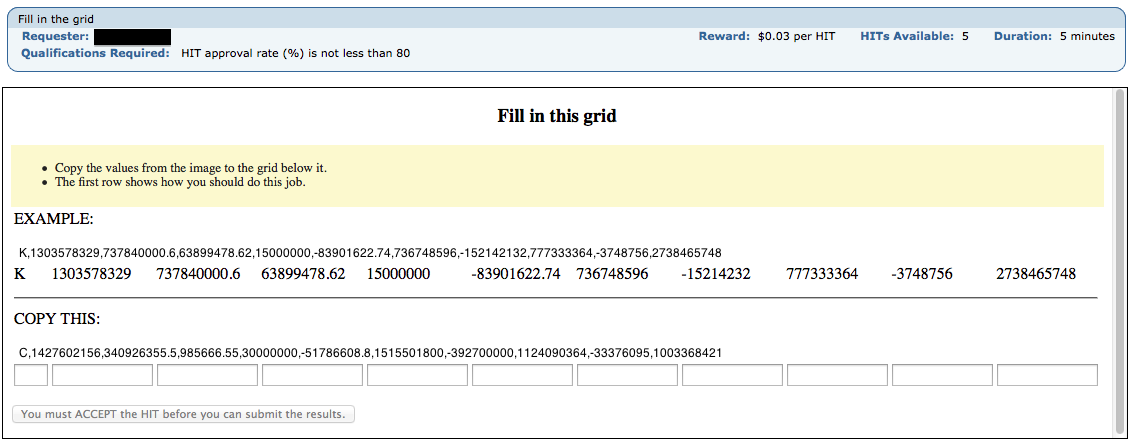
\includegraphics[width=5.5in]{images/mturk_fuzz_task}
  \caption{The page presented to Mechanical Turk workers to perform data entry tasks in order to collect actual human data entry errors (see Section~\ref{sec:user_study}).\label{fig:mturk_task}}
\end{figure*}


\begin{figure*}[!t]
\centering
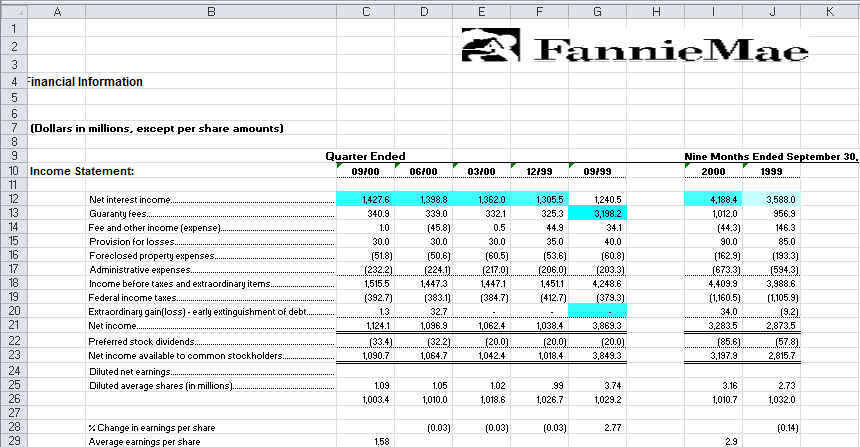
\includegraphics[width=5.5in]{images/fannie_mae_outlier}
  \caption{A screenshot of \checkcell{}'s results. In addition to the top row, which has a large impact on the final results, \checkcell{} highlights cell \texttt{G19}, a human data entry error.\label{fig:fannie_mae}}
\end{figure*}

Figure~\ref{fig:fannie_mae} presents a screenshot of \checkcell{}'s
results with one of these errors. In addition to the top
row, \checkcell{} indicates that cell \texttt{G19} has an unusual
impact; this is, in fact, the error. The correct value
for \texttt{G19} is \texttt{-379300000}, and the value entered by the
worker was \texttt{3793000000}: the worker made both a sign error and
an order of magnitude error (one too many 0's).

\paragraph{Summary:} By searching for data with unusual impacts on the spreadsheet, \checkcell{} is able to successfully find actual human data entry errors.




\section{Related Work}
\label{sec:related}
% The formula here is: discuss related work in one facet; end with a contrast with the current work.

\paragraph{Data Cleaning.}
Most past work on locating or removing errors in data has focused
on \emph{data cleaning} (also known as \emph{data scrubbing}
and \emph{cleansing}) in database
systems~\cite{DBLP:journals/debu/RahmD00,han2006data}. Standard
approaches include statistical outlier analysis for removing noisy
data~\cite{1583581}, interpolation to fill in missing data (e.g., with
averages), and using cross-correlation with other tables to correct or
locate errors~\cite{Hernandez:1995:MPL:223784.223807}.

% Also: noise removal.

% Section~\ref{FIXME} shows that statistical outlier analysis often produces unacceptably large numbers of false positives. 

% SURVEY! http://www.dbis.informatik.hu-berlin.de/dbisold/research/bioinformatics/papers/data_cleansing.html

A number of approaches have been developed that allow data cleaning to
be expressed programmatically or applied interactively. Programmatic
approaches include AJAX, which expresses a data cleaning program as a
DAG of transformations from input to
output~\cite{Galhardas:2000:AED:342009.336568}. Data Auditor applies
rules and target relations entered by a
programmer~\cite{Golab:2010:DAE:1920841.1921060}. A similar
domain-specific approach has been employed for data streams to smooth
data temporally and isolate it spatially~\cite{1617508}. Potter's
Wheel, by Raman and Hellerstein, is an interactive tool that lets
users visualize and apply data cleansing
transformations~\cite{Raman:2001:PWI:645927.672045}. 
Luebbers et al. describe an interactive data mining approach based on
machine learning that builds decision trees from databases. It marks
deviations from derived logical rules (e.g., ``$\mbox{BRV} =
404 \Rightarrow \mbox{GBM} = 901$'') as errors to be examined by a
data quality engineer~\cite{Luebbers:2003:SDD:1315451.1315499}.

Unlike these approaches, data debugging operates entirely
automatically (without the need for programmer-supplied rules or
latent logical relations in data) by measuring the interaction of data
with the programs that operate on them.
 

\paragraph{Spreadsheet Errors.}
Spreadsheets have been one of the most prominent computer applications
since their creation in 1979.
 The most widely used spreadsheet application today is Microsoft
Excel. Excel includes rudimentary error detection including errors in
formula entry like division by zero, a reference to a non-existient
formula or cell, invalid numerical arguments, or accidental mixing of
text and numbers.
% http://office.microsoft.com/en-us/excel-help/find-and-correct-errors-in-formulas-HP010066255.aspx
Excel also checks for inconsistency with adjacent formulas and other
structural errors, which it highlights with a ``squiggly'' underline. In addition, Excel provides a formula auditor, which lets spreadsheet view dependencies flowing into and out of a particular formula.
% http://office.microsoft.com/en-us/excel-help/use-error-checking-to-correct-common-errors-in-formulas-HA010342331.aspx

Past work on detecting errors in spreadsheets has focused on inferring
units and relationships (has-a, is-a) from information like layout and
headers~\cite{DBLP:conf/kbse/AhmadAGK03}. XeLda checks if formulas
process values with incorrect units or if derived units clash with
unit annotations~\cite{Antoniu:2004:VUC:998675.999448}.  More type
system stuff:~\cite{Erwig:2005:AGM:1062455.1062494}. Using labels and
structural clues (especially unit-of-measurement
errors)~\cite{Chambers:2010:RSL:1860134.1860346}. There also has been
considerable work on testing tools for
spreadsheets~\cite{fisher2006scaling,rothermel1998you,rothermel2001methodology,Carver:2006:EET:1159733.1159775}). Much
of this work is complementary and orthogonal to \checkcell{}, which
works with standard, unannotated spreadsheets and focuses on unusual
interactions of data with formulas.


% What is Jaffry et al\. ~\cite{DBLP:journals/corr/abs-0803-1748}?

\paragraph{Outlier Analysis}

Techniques to remove outliers (unusual data) date to the earliest days
of statistics, when they were developed to make nautical measurements
more robust. Widely-used approaches include Peirce's criterion,
Chauvenet's criterion, and Grubb's test for outliers~\cite{barnett1994outliers}. All
of these techniques require that data belong to a known distribution,
primarily the normal (Gaussian). Unfortunately, input data does not
always fit any statistical distribution. Even when outlier detection is
possible, identifying them leads to false positives when they do not
materially contribute to the result of a computation.
\checkcell{} leverages the
fact that its statistical sampling approach forces observed effects to
follow a Gaussian distribution (as Section~\ref{sec:FIXME} explains),
allowing it to use the Peirce outlier test to determine whether a
particular value has an unusual impact on a computation.



\section{Future Work}
\label{sec:future}
Future work.


\section{Conclusion}
\label{sec:conclusion}
\section{Summary}

\todo{Timeline}

We propose data debugging, an approach aimed at
finding potential data errors by locating and ranking data items based on their
overall impact on a computation. Intuitively, errors that have no
impact do not pose a problem, while values that have an unusual impact
on the overall computation are either very important or incorrect.
We present a prototype of the first data debugging
tool, \checkcell{}, which operates on spreadsheets. We evaluate
\checkcell{}'s performance analytically and empirically, showing that
it is reasonably efficient and effective at helping to find data
errors. \emph{FIX ME.}




%\appendix
%\section{Appendix Title}

% This is the text of the appendix, if you need one.

%\acks

% \bibliographystyle{abbrvnat}

% The bibliography should be embedded for final submission.
{
\bibliographystyle{abbrv}
\bibliography{ref}
}

\end{document}
